\documentclass[10pt]{article}
\usepackage{geometry}                
\geometry{a4paper}                  
\usepackage[parfill]{parskip}    
\setlength{\parskip}{0pt}
\usepackage{graphicx}
\usepackage{amssymb}


\title{Software Engineering Assessed Exercise 1}
\author{Paul McHard - 2085227M}
\date{}
\begin{document}
\maketitle

\subsubsection*{Introduction}The aim of this assessed exercise is to develop multiple UML design diagrams for a simple word processing program in Java. The desired core functionality and data to be handled was provided as part of a \textbf{User Requirements Specification.} The desired end product must provide the functionality for: \textit{Document File Management}, a \textit{Graphical WYSIWYG Interface} and \textit{Document and Text Customisation}. The system must be capable of allowing users to create new documents, to open, edit and save new and existing documents and manipulate font size, colour and typeface, and save stylings for multiple uses. The GUI must also be sufficient to allow users to access the processor's other functionalities. Three implementations are desired; the first must be optimised for absolute reduction of coupling, the second optimised for absolute increase in cohesion and the last must strike a balance between the two. Ideally a program should seek to implement a design which employs highly cohesive objects which are not strongly coupled together.

\subsubsection*{Assumptions}
\begin{itemize}
\item{It is assumed that accessor methods for private variables within classes do not need to be shown. These are not shown in example UML class diagrams found in O.O.S.E. \emph{(Lethbridge and Laganiere, 2nd Ed.)}\cite{oose}, and it is assumed this textbook is the intended reference for this exercise.}
\item{It is also assumed that a class which exists only to provide the \emph{main} method required to execute the program in Java need not be shown in these diagrams, as it is likewise excluded from UML class diagrams in O.O.S.E.\cite{oose}}
\item{It is further assumed that non-functional GUI elements, such as Frames and Panels, which would be required for an actual implementation of the system are not required to be detailed in the diagrams put forward in this report.}
\item{It is assumed that the models discussed should not aim to functionally exceed the \textbf{User Requirements Definition} provided.}
\end{itemize}

\subsubsection*{First Solution - Reduce Coupling}Coupling is unfortunately inherent of Object Oriented Programming in systems above a trivial simplicity. Some coupling, primarily \emph{Routine Call, Data} and, to an extent, \emph{Stamp Coupling}, is required for communication between objects in the system. Other forms of coupling, such as \emph{Common, Content} or \emph{Type Use Coupling}, can be entirely removed from the design; these forms are rarely necessary and can potentially damage the function and security of the system. It is important to acknowledge that some coupling must exist for the system to function, and appreciate that there are good and bad types of coupling which can occur. \newline

In this solution I have aimed to reduce coupling by implementing an interface, \texttt{EditorInterface}, through which all editing and file management operations are implemented. This reduces coupling to the \texttt{Document} object and its components, as the Document cannot \textit{see} which implementation it is interacting with. Therefore any future classes added which implement the interface will not affect the relationship with the Document. Additionally, the use of the Observer pattern is helpful in reducing coupling, particularly in situations such as this where there is association between an object which updates another whenever change occurs, ie. the document view that the user sees.

\begin{figure}[h]
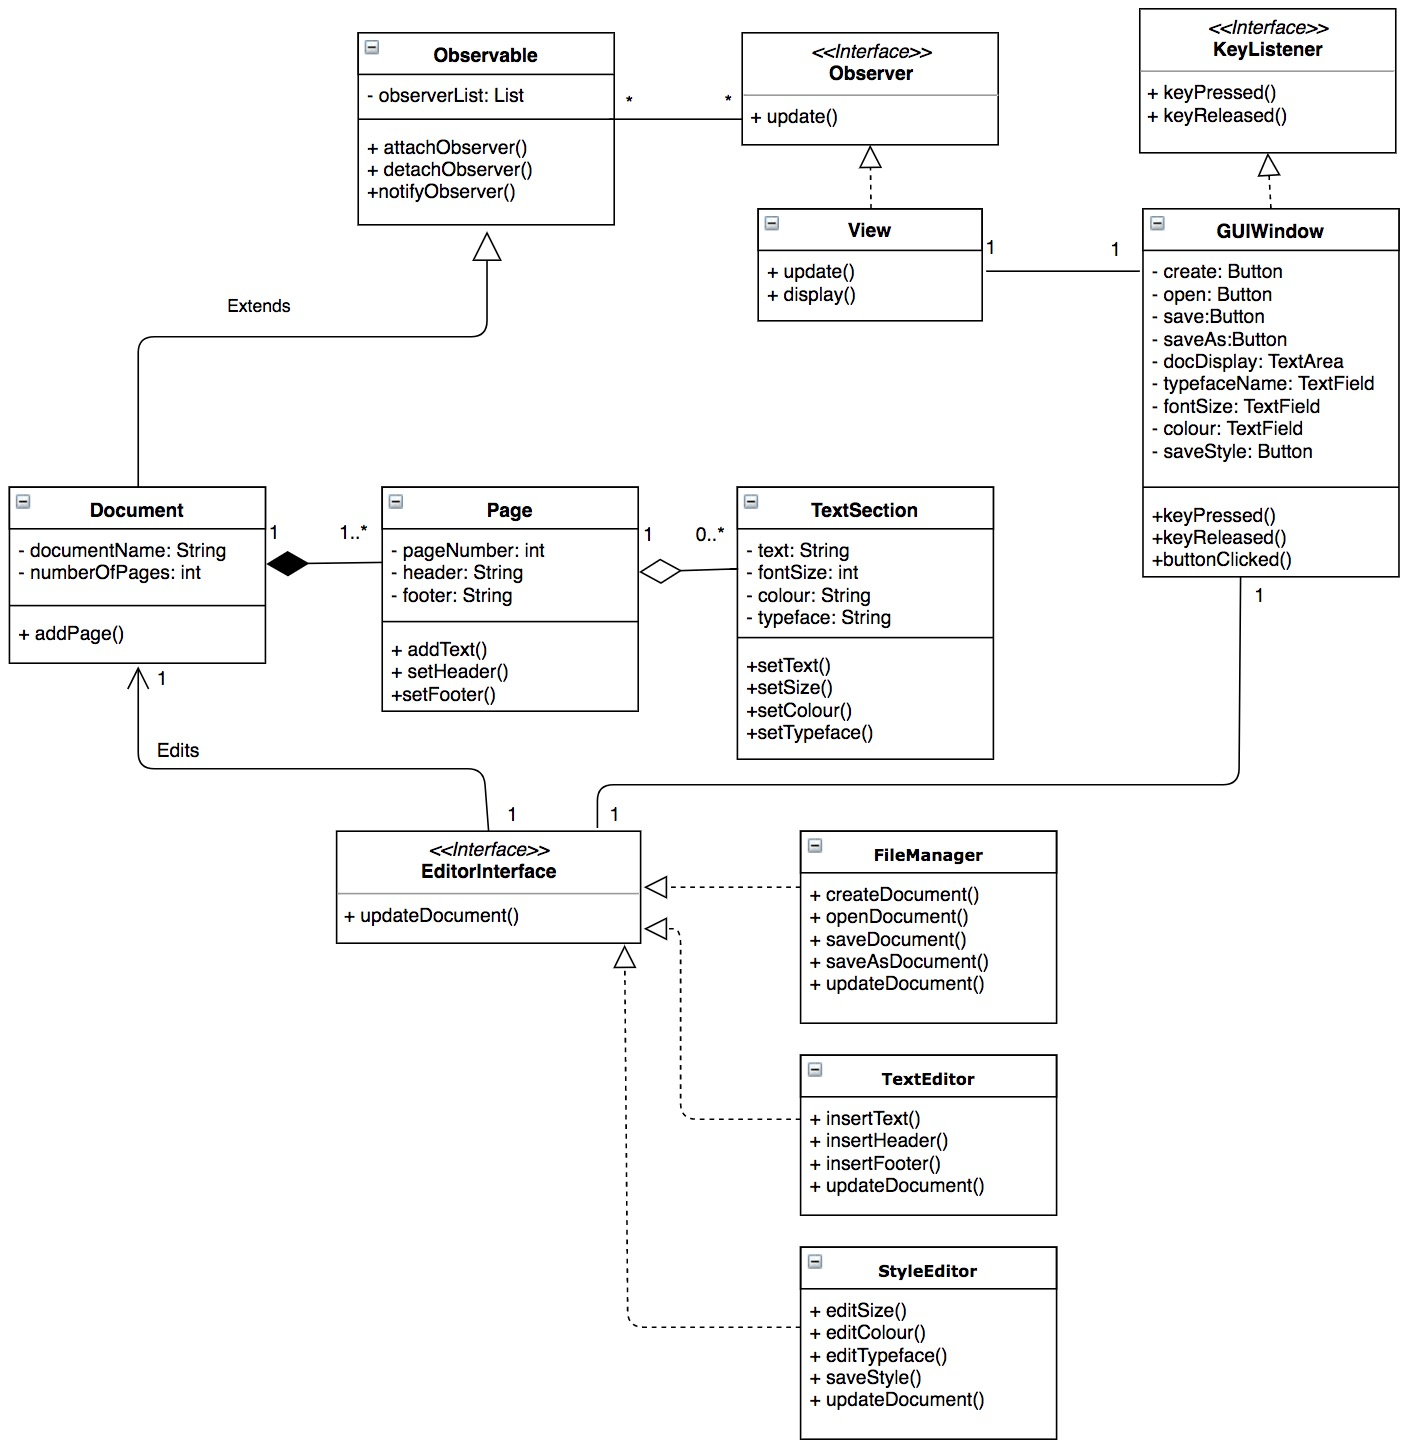
\includegraphics[width=0.8\textwidth]{reducedCoupling5}
\centering
\caption{Solution with focus on reducing coupling.}
\end{figure}

\subsubsection*{Second Solution - Increase Cohesion}Cohesion refers to the focus a class or module has on its task. Code designed to be highly cohesive uses the divide and conquer principle in an intelligent way to split code into concise classes and modules which handle only relevant data. This can resultantly lead to reduced coupling.\newline

In this solution I have aimed to demonstrate my understanding of design which increases cohesion at the expense of low coupling, to provide a solution which significantly contrasts my first. Hence why I have chosen to demonstrate the Facade pattern; this design can be used to ensure that each class which performs an operation on the document has exactly its required amount of methods without any excess.This also results in a system which is easier to use by the client. It is less dependent on other packages, and so \emph{external} coupling would ultimately be low once implemented in Java. The main limitation of this system is that it increases \emph{internal} coupling within the system when compared to the first solution. Implementing the Facade as a singleton pattern, ensuring it can only be called once, maintains cohesion by preventing repeated implementation.

\begin{figure}[h]
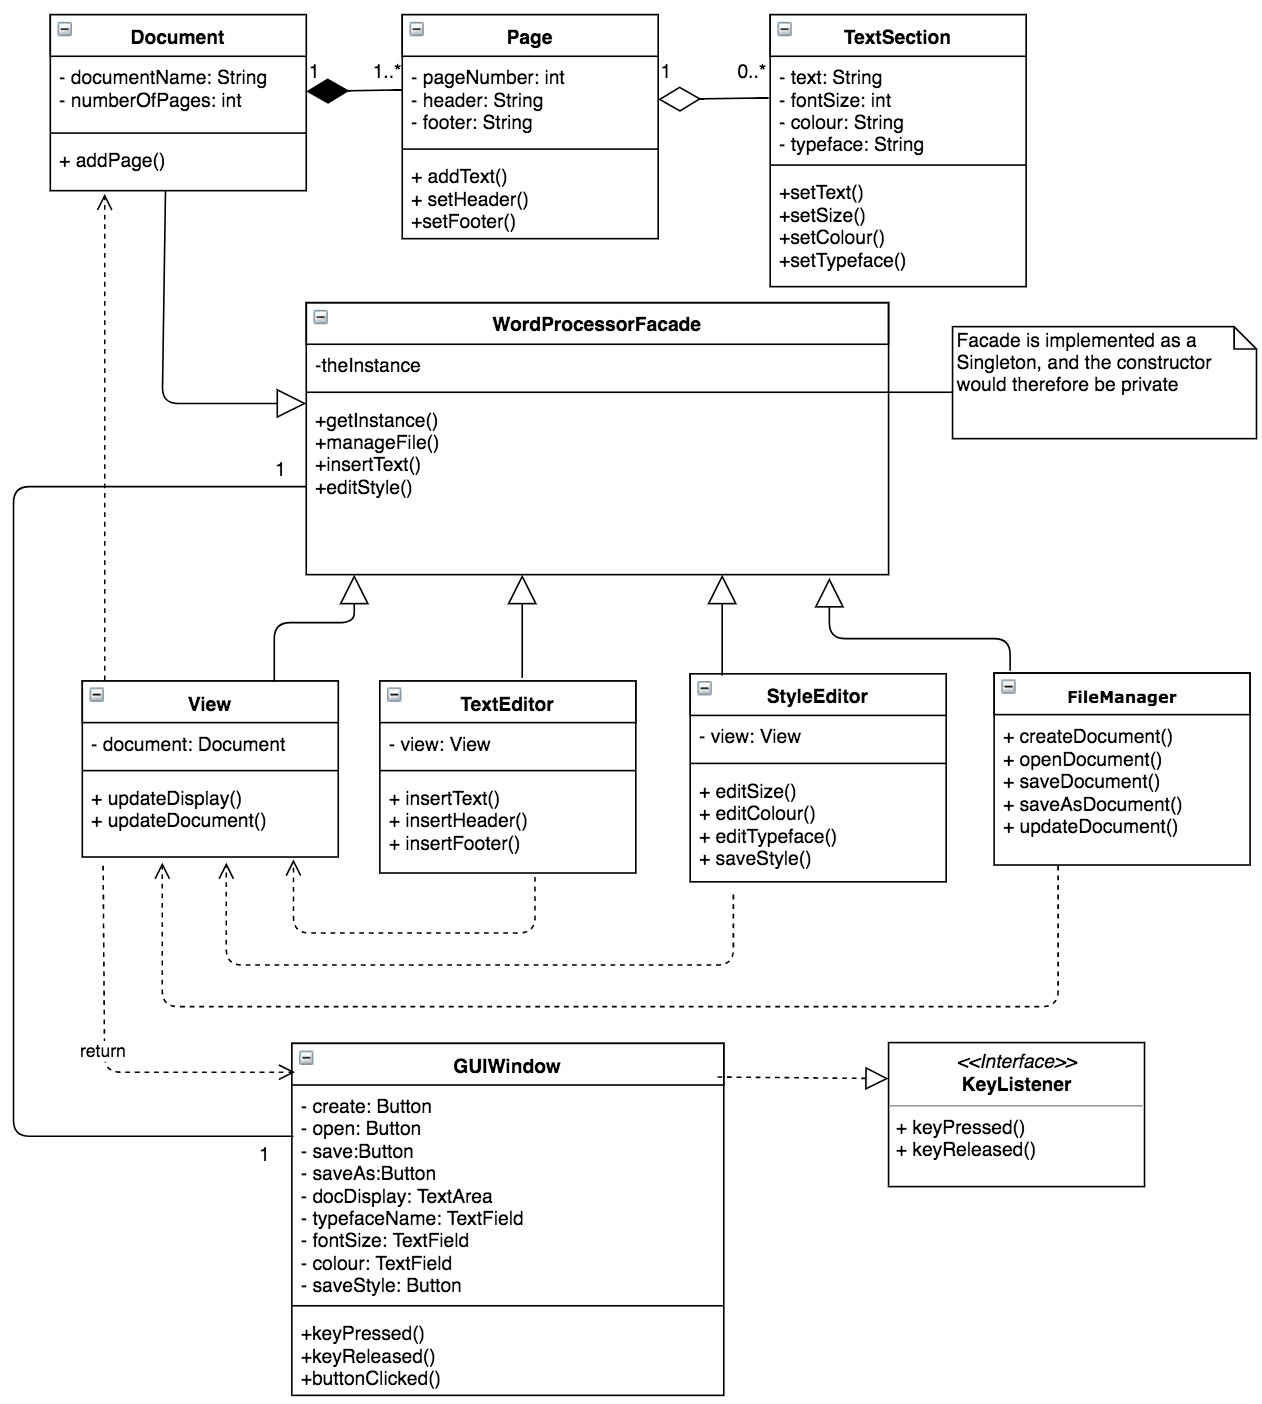
\includegraphics[width=0.8\textwidth]{increasedCohesion5}
\centering
\caption{Solution with focus on increasing cohesion.}
\end{figure}

\subsubsection*{Third Solution - Balance of High Cohesion and Low Coupling}
Lastly, I present my final design. To meet the aim of balancing increased cohesion with reduced coupling and find an optimal system, I feel the best approach is to utilise the \emph{Model-View-Controller} architecture. MVC architecture is designed with the principle of divide and conquer in mind. As I have discussed previously, this principle facilitates high cohesion, demonstrated by the separation of logic, view and control in this pattern; each level of the framework is separated, and focussed on its purpose. While this doesn't match the cohesive partitioning of the Facade, it still provides functionally high cohesion. \newline

Similarly to my first solution, I have implemented an interface, \texttt{EditorInterface}, which falls under the \emph{View} when incorporated into the MVC architecture. As before, this facilitates reduced coupling and is well suited to use within the MVC architecture. Coupling in this system can be reduced to only what is necessary for communication between the three components  of the system. The main limitation of this design is that it's potentially unnecessarily bulky for the scope of the application required, however, it sets the framework well to limit coupling and promote cohesion if the system were to be expanded to be more sophisticated.
\begin{figure}[h]
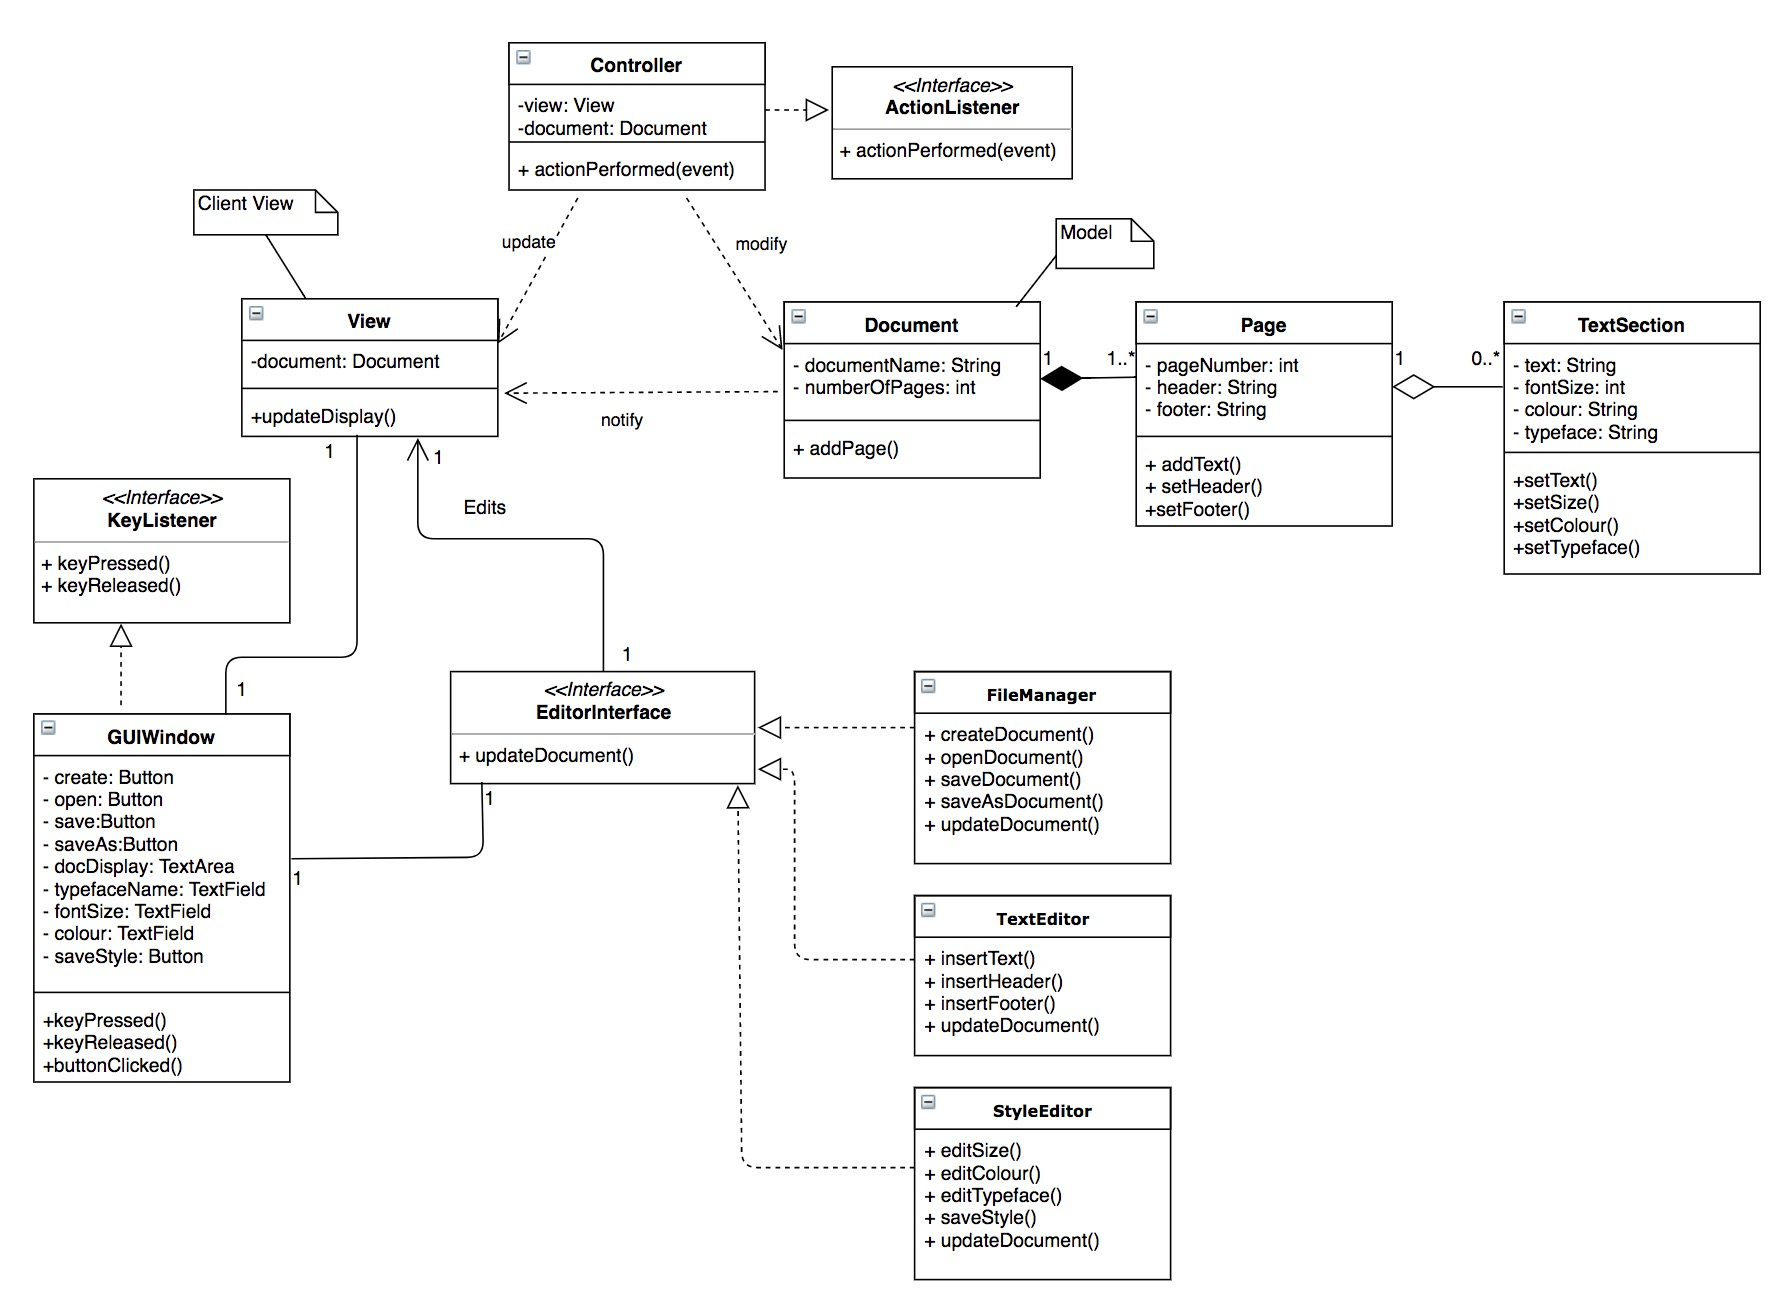
\includegraphics[width=0.9\textwidth]{balancedSolution4}
\centering
\caption{Balanced Solution.}
\end{figure}

\begin{thebibliography}{1}
\bibitem{oose}
Timothy Lethbridge and Robert Lagani�re. 
\textit{Object-oriented software engineering.} 
New Delhi: Tata McGraw-Hill, 2007.
\end{thebibliography}
\end{document}  